\documentclass{article}
\title{ECO206 Lecture Notes}
\author{Tianyu Du}
\date{\today}

% Libraries.
\usepackage{amsmath}
\usepackage{amssymb}
\usepackage{pgfplots}
\usepackage{graphicx}
\usepackage{enumitem}
\usepackage{hyperref}
\usepackage{fancyhdr}
\usepackage{perpage}
\usepackage{float}

% Property settings.
\MakePerPage{footnote}
\pagestyle{fancy}
\lhead{Notes by T.Du}
\usepackage[
	type={CC},
	modifier={by-sa},
	version={3.0},
]
{doclicense}

% Attr.
\title{ECO206 Microeconomic Theory \\ Lecture Notes}
\author{Tianyu Du}
\date{\today}
% Macro
\newcommand{\trans}[3]{{#1}: {#2} \to {#3}}
\newcommand{\R}[0]{\mathbb{R}}
\newcommand{\M}[2]{\mathbb{M}_{{#1} \times {#2}}(\mathbb{R})}
\newcommand{\coor}[2]{[\vec{{#1}}]_{{#2}}}
\newcommand{\tmat}[3]{[{#1}]_{{#2}}^{{#3}}}
\newcommand{\vset}[3]{\{\vec{{#1}_{#2}}, \dots, \vec{{#1}_{#3}}\}}
\newcommand{\sset}[3]{\{{{#1}_{#2}}, \dots, {{#1}_{#3}}\}}
\newcommand{\definition}[0]{\paragraph{Definition}}
\newcommand{\theorem}[0]{\paragraph{Theorem}}
\newcommand{\C}[0]{\mathbb{C}}
\newcommand{\restrans}[2]{{#1}\vert_{#2}}
\newcommand{\tx}[1]{\text{{#1}}}
\newcommand{\pd}[2]{\frac{\partial {#1}}{\partial {#2}}}


\begin{document}
	\maketitle
	\doclicenseThis
	\tableofcontents
	
	
	\section{Lecture 1 May. 8 2018}
	\subsection{Budget Constraint}
	\begin{itemize}
		\item Exogenous income
		\item Endogenous income:
	\end{itemize}
	\paragraph{Bundle} Combination of goods. If we have $n$ goods, then $x_1^A$ represents a quantity ($x$) of good $1$ in bundle $A$.
	\[
		A = (x_1^A, x_2^A, \dots, x_n^A)
	\]
	
	\begin{figure*}[!htb]
		\centering
		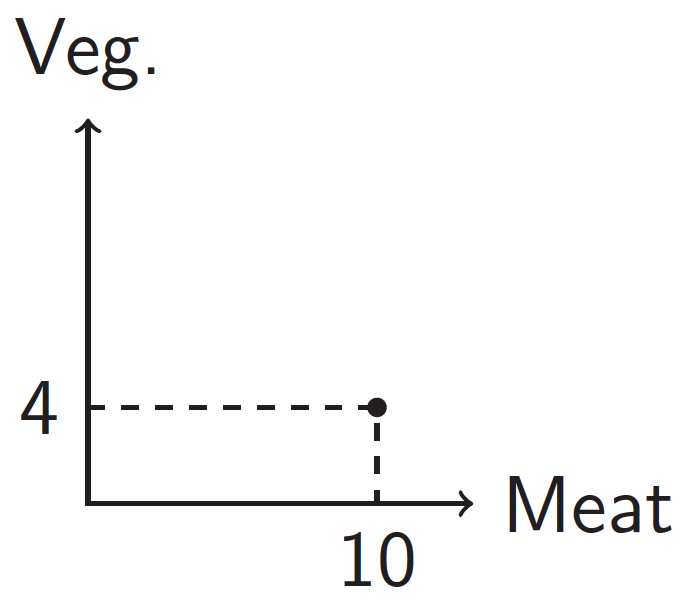
\includegraphics[width=0.3\linewidth]{eco206pic/bundle}
		\caption{Consumption bundle}
	\end{figure*}
	
	\subsubsection{Types of Income}
	\paragraph{Exogenous income}Cash(i.e. $\$$) in your pocket to spend.
	\paragraph{Endogenous income}Bundle fo goods you can sell to get money. e.g. \emph{Assets}, \emph{Skills}, \emph{Time}, etc.
	\subsubsection{Exogenous Income} Consumer walk into market with a fixed amount of \textbf{cash}, budget constraint.
	\[
	\vec{x} \cdot \vec{p} \leq I
	\]
	\begin{figure*}[!htb]
		\centering
		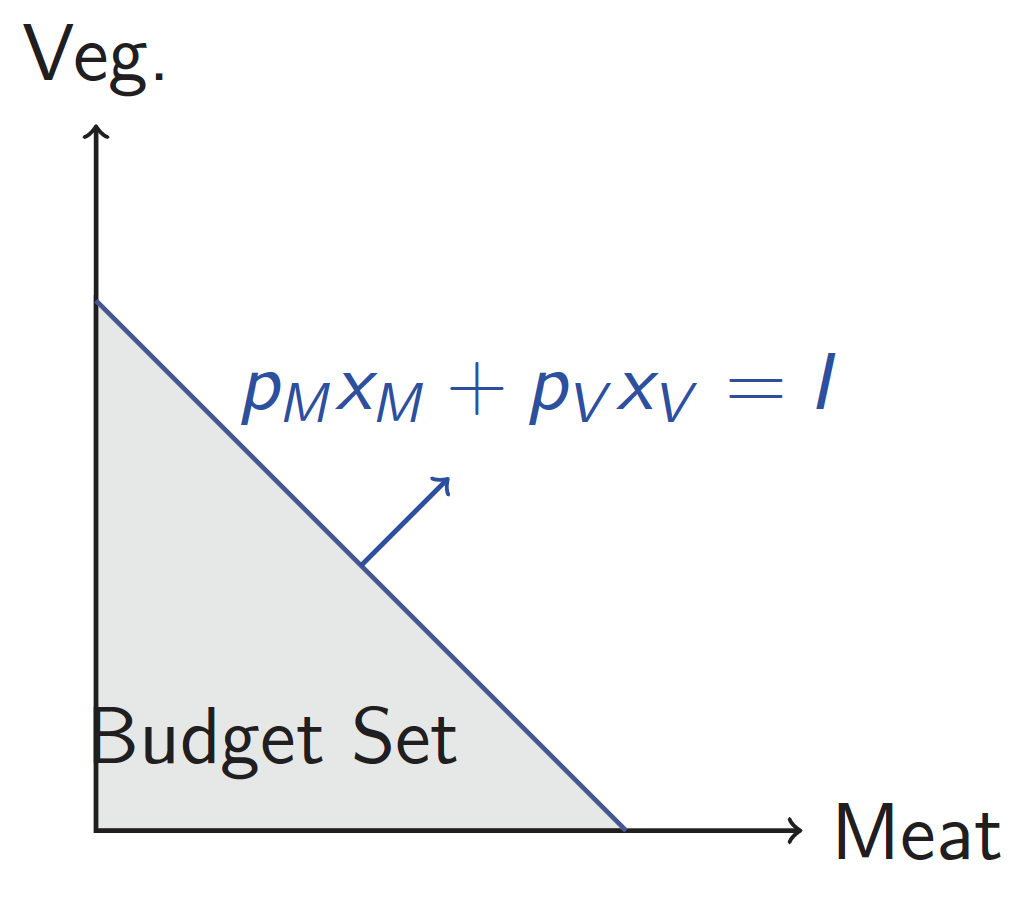
\includegraphics[width=0.3\linewidth]{eco206pic/budget}
		\caption{Budget constraint}
	\end{figure*}
	
	\subsubsection{Endogenous Income}
	\paragraph{Framework} Consumer walks into a market \textbf{without cash}, but with \textbf{endowment} $(\omega_M, \omega_V)$. And consumer can sell the endowment at market prices, the \underbar{value of the endowment} is
	\[
		p_M \omega_M + p_V \omega_V
	\]
	\paragraph{Hypothetical income} Income/Cash from selling the \emph{entire} bundle endowed. 
	\paragraph{Budget Constraint equation}
	\[
		p_M x_M + p_V x_V \leq I_{hypothetical} = p_M \omega_M + p_V \omega_V
	\]
	Intercepts: if spend all income on one good.
	\begin{itemize}
		\item x-axis(meat) = $\frac{p_M \omega_M + p_V \omega_V}{p_M} = \omega_M + \frac{p_V}{p_M}\omega_V$
		\item y-axis(veg) = $\frac{p_M \omega_M + p_V \omega_V}{p_V} = \omega_V + \frac{p_M}{p_V}\omega_M$
	\end{itemize}
	\paragraph{Assumption} consumers are price takers.
	\paragraph{Affordable} means $spending \leq income$ and $\vec{x} \in \mathbb{R}^n_{+}$
	\subsection{Opportunity Cost}
	\paragraph{OC/MRT} Rate at which one good can be traded for another though the market, \underbar{expressed in units of a good}.
	
	\emph{To get another \underbar{unit} of good 1 home many \underbar{unit} of good 2 do I need to give up?}
	\[
		\frac{dy}{dx} = -\frac{p_x}{p_y}
	\]
	\subsection{Changes that affect the budget constraint}
	\subsubsection{Pure income change} keeping relative prices constant. i.e. $\frac{p_1}{p_2} = \overline{p}$
	\begin{figure*}[h]
		\centering
		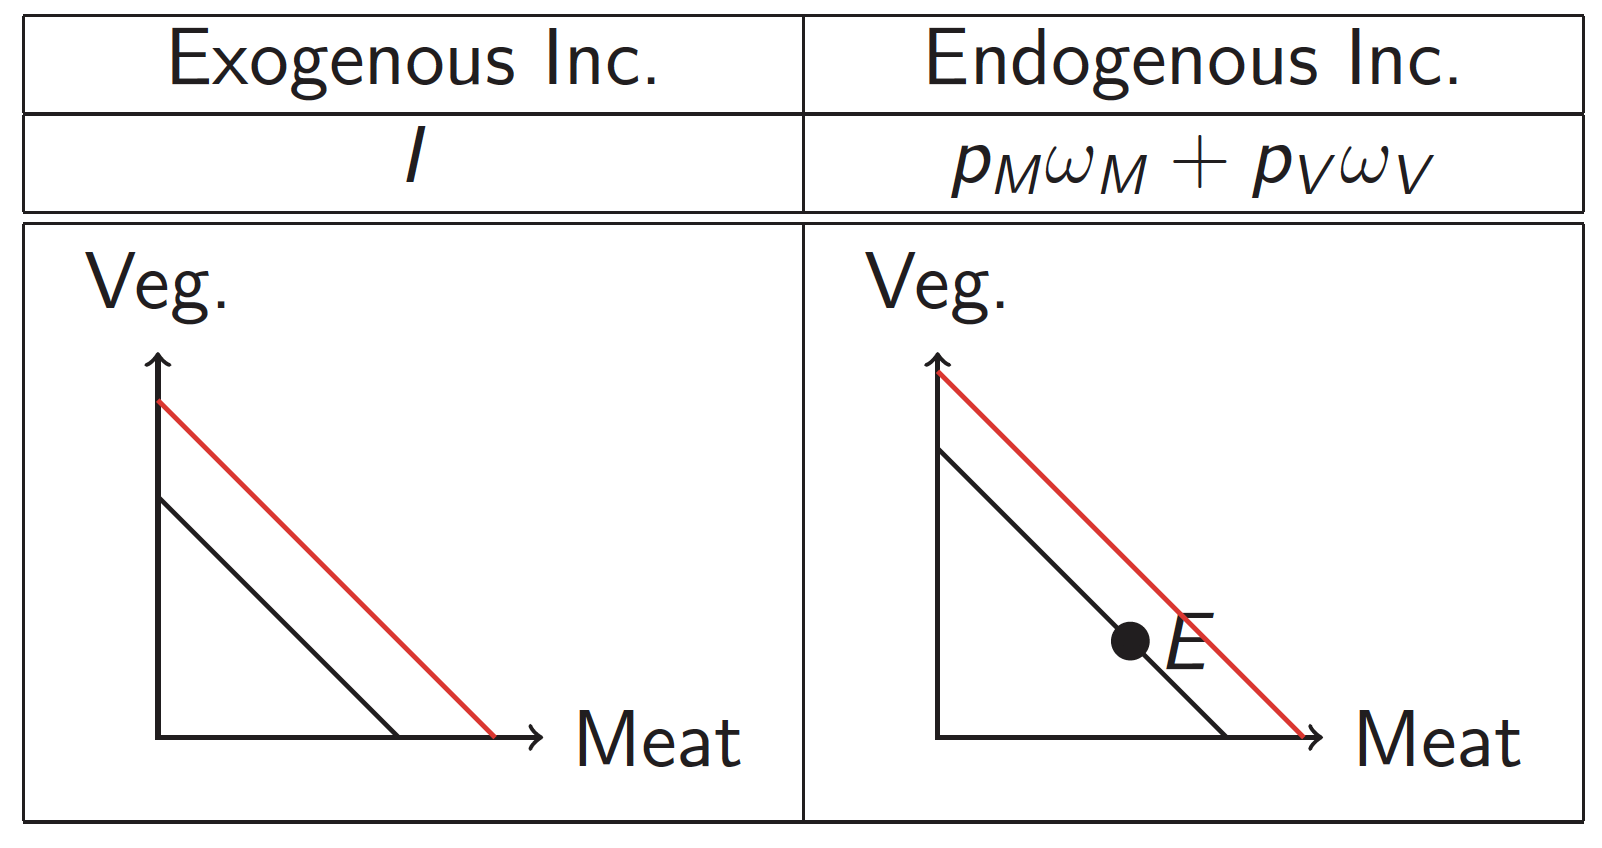
\includegraphics[width=0.5\linewidth]{eco206pic/income_change}
		\caption{Pure income change}
	\end{figure*}
	
	
	\textbf{Note} Changes in prices(relative price holds) will change the budget constraint in exogenous income budget, but will \emph{not} affect the endogenous income constraint.
	
	\textbf{Conclusion} To change budget constraint defined with endogenous income, we need \textbf{endowment changes}.
	
	\subsubsection{Price change}
	\begin{figure*}[!htb]
		\centering
		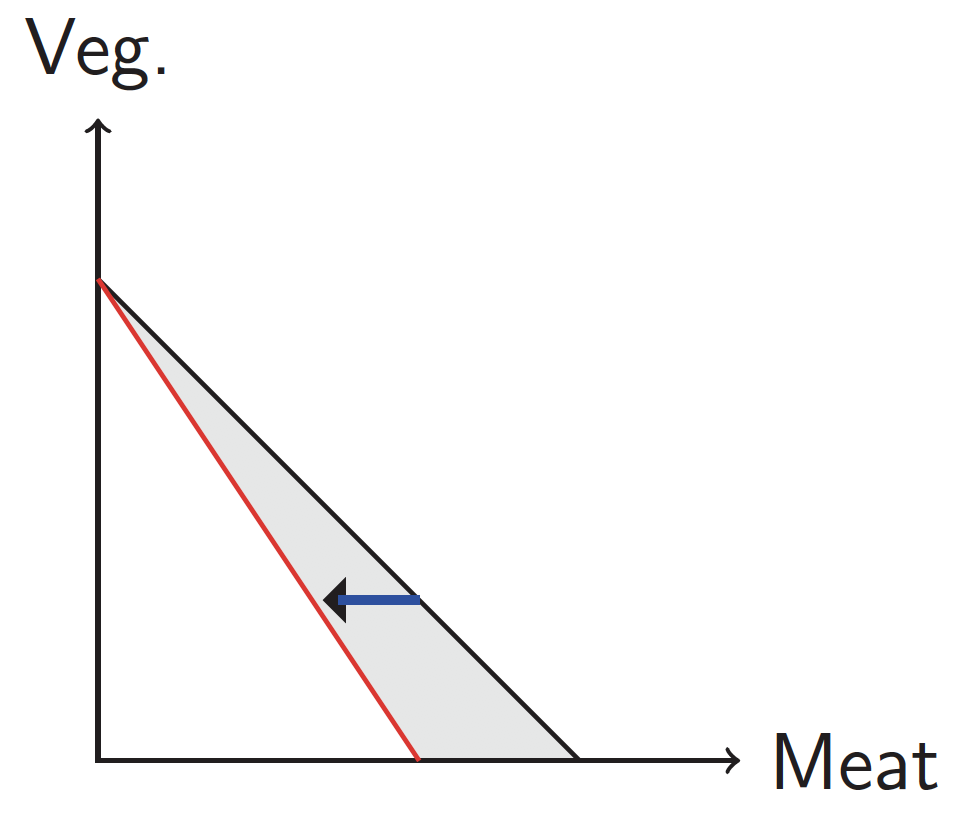
\includegraphics[width=0.5\linewidth]{eco206pic/relative_price_change}
		\caption{Relative price change}
	\end{figure*}
	
	\subsubsection{Endogenous income price change}
	\paragraph{Intuition} \textbf{Rotation} about the endowment.
	\begin{figure*}[!htb]
		\centering
		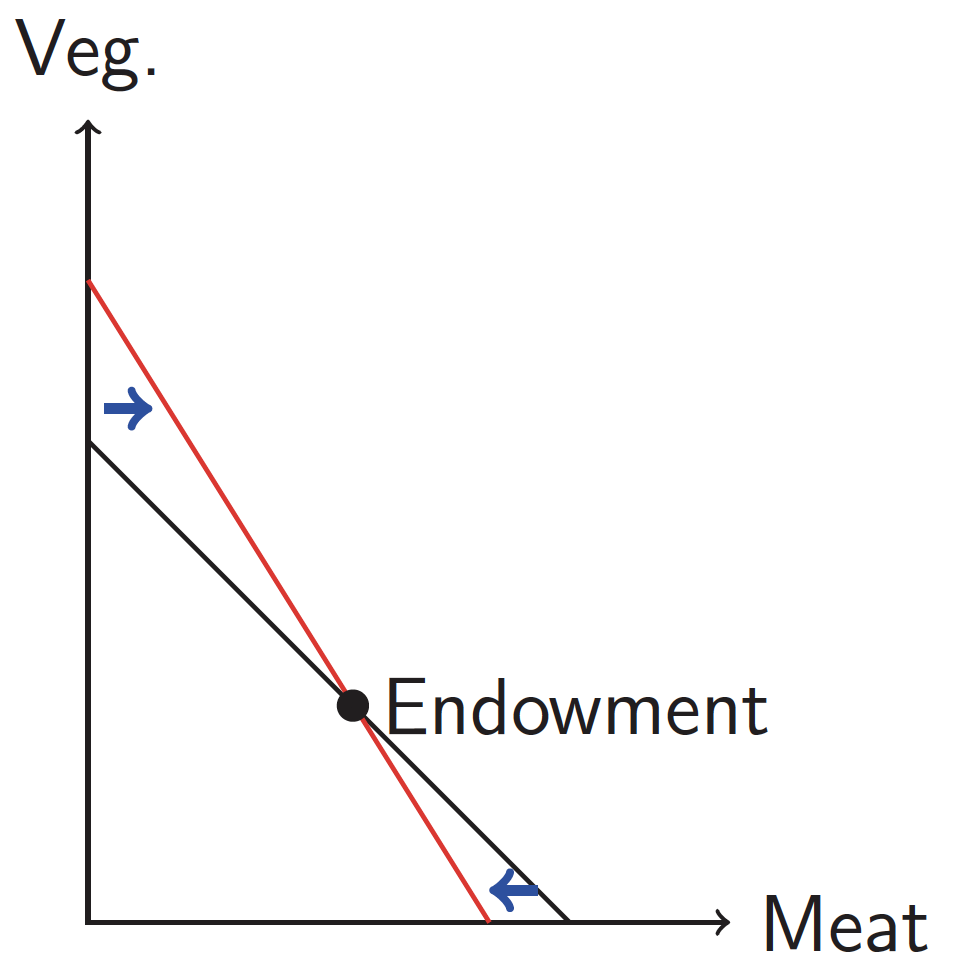
\includegraphics[width=0.5\linewidth]{eco206pic/End_price_change}
		\caption{Endogenous income price change}
	\end{figure*}
	

\section{Lecture 2 May. 9 2018}
\paragraph{Tophat} Assume endogenous income and 2 goods - meat and vegetables. When the price of meat goes up, can you afford more bundles? Explain your reasoning briefly.

\textbf{Key points}
\begin{enumerate}
	\item Relative price $\rightarrow$ Exchange rate.
	\item Holding fixed amount of meat, consider the quantity of veg could be consumed.
	\item Endowment point.
\end{enumerate}

\subsection{Tastes as Binary Relations}
\paragraph{Strictly preferred} Consider bundles $A=(x_1^A, x_2^A)$ and $B=(x_1^B, x_2^B)$, we denote \underbar{Bundle $A$ is strictly preferred as $B$} as,
\[
	(x_1^A, x_2^A) \succ (x_1^B, x_2^B)
\]

\paragraph{At least as good as} Consider bundles $A=(x_1^A, x_2^A)$ and $B=(x_1^B, x_2^B)$, we denote \underbar{Bundle $A$ is at least as good as $B$} as,
\[
	(x_1^A, x_2^A) \succcurlyeq (x_1^B, x_2^B)
\]
\paragraph{Indifference} Consider bundles $A=(x_1^A, x_2^A)$ and $B=(x_1^B, x_2^B)$, we denote \underbar{Bundle $A$ is indifferent to $B$} as,
\[
	(x_1^A, x_2^A) \sim (x_1^B, x_2^B)
\]

\subsection{Rationality Assumptions on Preference Relation}

\paragraph{Completeness} Let $X$ denote the consumption set, then we say a preference relation $\succcurlyeq$ satisfies \underbar{completeness} if and only if
\[
	\forall \vec{x_1}, \vec{x_2} \in X,\ \vec{x_1} \succcurlyeq \vec{x_2} \lor \vec{x_1} \preccurlyeq \vec{x_2}
\]

\paragraph{Transitivity} Let $X$ denote the consumption set, then we say a preference relation $\succcurlyeq$ satisfies \underbar{transitivity} if and only if
\[
	\forall \vec{x_1}, \vec{x_2}, \vec{x_3} \in X,\ (\vec{x_1} \succcurlyeq \vec{x_2} \land \vec{x_2} \succcurlyeq \vec{x_3}) \implies \vec{x_1} \succcurlyeq \vec{x_3}
\]

\paragraph{Rational tastes} If those two assumption hold, we say the individual has \underbar{rational tastes}.

\subsection{Convenience Assumptions}
\paragraph{(Strict) Monotonicity} Let $X$ denote the consumption set, a preference relation $\succcurlyeq$ satisfies \underbar{monotonicity} if and only if
\[
	\forall \vec{x_1}, \vec{x_2} \in X,\ (\vec{x_1} \geq \vec{x_2} \implies \vec{x_1} \succcurlyeq \vec{x_2}) \land (\vec{x_1} \gg \vec{x_2} \implies \vec{x_1} \succ \vec{x_2})
\]

\paragraph{(Weak) Convexity} \emph{Intuitively, Averages are better than extremes, or at least
no worse.} Let $X$ denote the consumption set, a preference relation $\succcurlyeq$ satisfies
\underbar{(weak) convexity} if and only if
\[
	\forall \vec{x_1}, \vec{x_2} \in X,\ \vec{x_1} \sim \vec{x_2} \implies \lambda \vec{x_1} + (1 - \lambda) \vec{x_2} \succcurlyeq \vec{x_1},\ \forall \lambda \in [0, 1]
\]

\paragraph{Continuity} \emph{Intuitively, no sudden preference switching},  mathematically, let consumption set $X \subseteq \mathbb{R}^n_{+}$, $\forall \vec{x} \in X,$ the "no better than" set, $\preccurlyeq(\vec{x})$ and the "no worse than" set, $\succcurlyeq(\vec{x})$ are closed in $\mathbb{R}^n_{+}$. \footnote{The mathematical definition is not required in ECO206.}

\subsection{Indifference Curve}
\paragraph{Definition} Let consumption bundle $A \in X \subseteq \mathbb{R}^n_{+}$, the \underbar{indifference curve} \underbar{corresponding to consumption bundle $A$} is defined as
\[
	\sim(A) = \{\vec{x} \in X\ \vert\ \vec{x} \sim A\}
\]

\paragraph{Properties}
\begin{enumerate}
	\item IC slopes downwards $\impliedby$ monotonicity.
	\item ICs does not cross (for individual preference).
	\item Direction of increasing preference.
\end{enumerate}

\subsection{Utility Function}
\paragraph{Definition} A \underbar{real-valued function} $u: \mathbb{R}^n_{+} \to \mathbb{R}$ is called a \textbf{utility function} representing the preference relation $\succcurlyeq$, if for all $\vec{x_0}, \vec{x_1} \in \mathbb{R}^n_{+}$, $u(\vec{x_0}) \geq u(\vec{x_1}) \iff \vec{x_0} \succcurlyeq \vec{x_1}$.

\paragraph{Marginal Rate of Substitution (MRS)} Consider the scenario with two commodities, intuitively, MRS could be interpreted as the quantity of one commodity must be forgone for one unit increment in the other commodity, holding the utility value constant. Graphically, MRS is the (absolute value of) slope of indifference curve. Mathematically, MRS can be computed as \footnote{The negative sign indicates \emph{forgoing}.}
\[
	\frac{dy}{dx} = - \frac{\frac{\partial u(\cdot)}{\partial x}}{\frac{\partial u(\cdot)}{\partial y}}
\]

\section{Lecture 3 May. 15 2018}
\subsection{Different Types of Tastes}
\paragraph{Questions}
\begin{itemize}
	\item How MRS changes \textbf{along} IC. (\emph{substitutability})
	\item How MRS changes \textbf{across} ICs.
\end{itemize}
\subsubsection{Shape and Substitutability Along IC}
\begin{center}
	\begin{tabular}{|c|c|}
		\hline
		Type & MRS \\
		\hline
		Perfect Substitutes & Constant \\
		\hline
		Perfect Complements & $\infty$ or $0$ or undefined \\
		\hline
		In Between & changes along IC \\
		\hline
	\end{tabular}
\end{center}

\subsubsection{Diminishing MRS}


\section{Tutorial 2 May. 17 2018}

\paragraph{MRS} In this course, defined \underbar{with} the minus sign.

\[
	MRS = \frac{dy}{dx}\vert_{u(x,y) = \overline{u}} = - \frac{\frac{\partial u}{\partial x}}{\frac{\partial u}{\partial y}}
\]

\subsection{Different types of utility functions}

\paragraph{Exercise1 (perfect complement)} Preference over violins (v) and strings (s). Consume 4 strings with every violin. Any extras are discarded and cannot be used.
\newline
(a) utility function.
\[
	u(v, s) = min\{4v, s\}
\]
\newline
(b) Graph an indifference curve
\begin{figure*}[!htb]
	\centering
	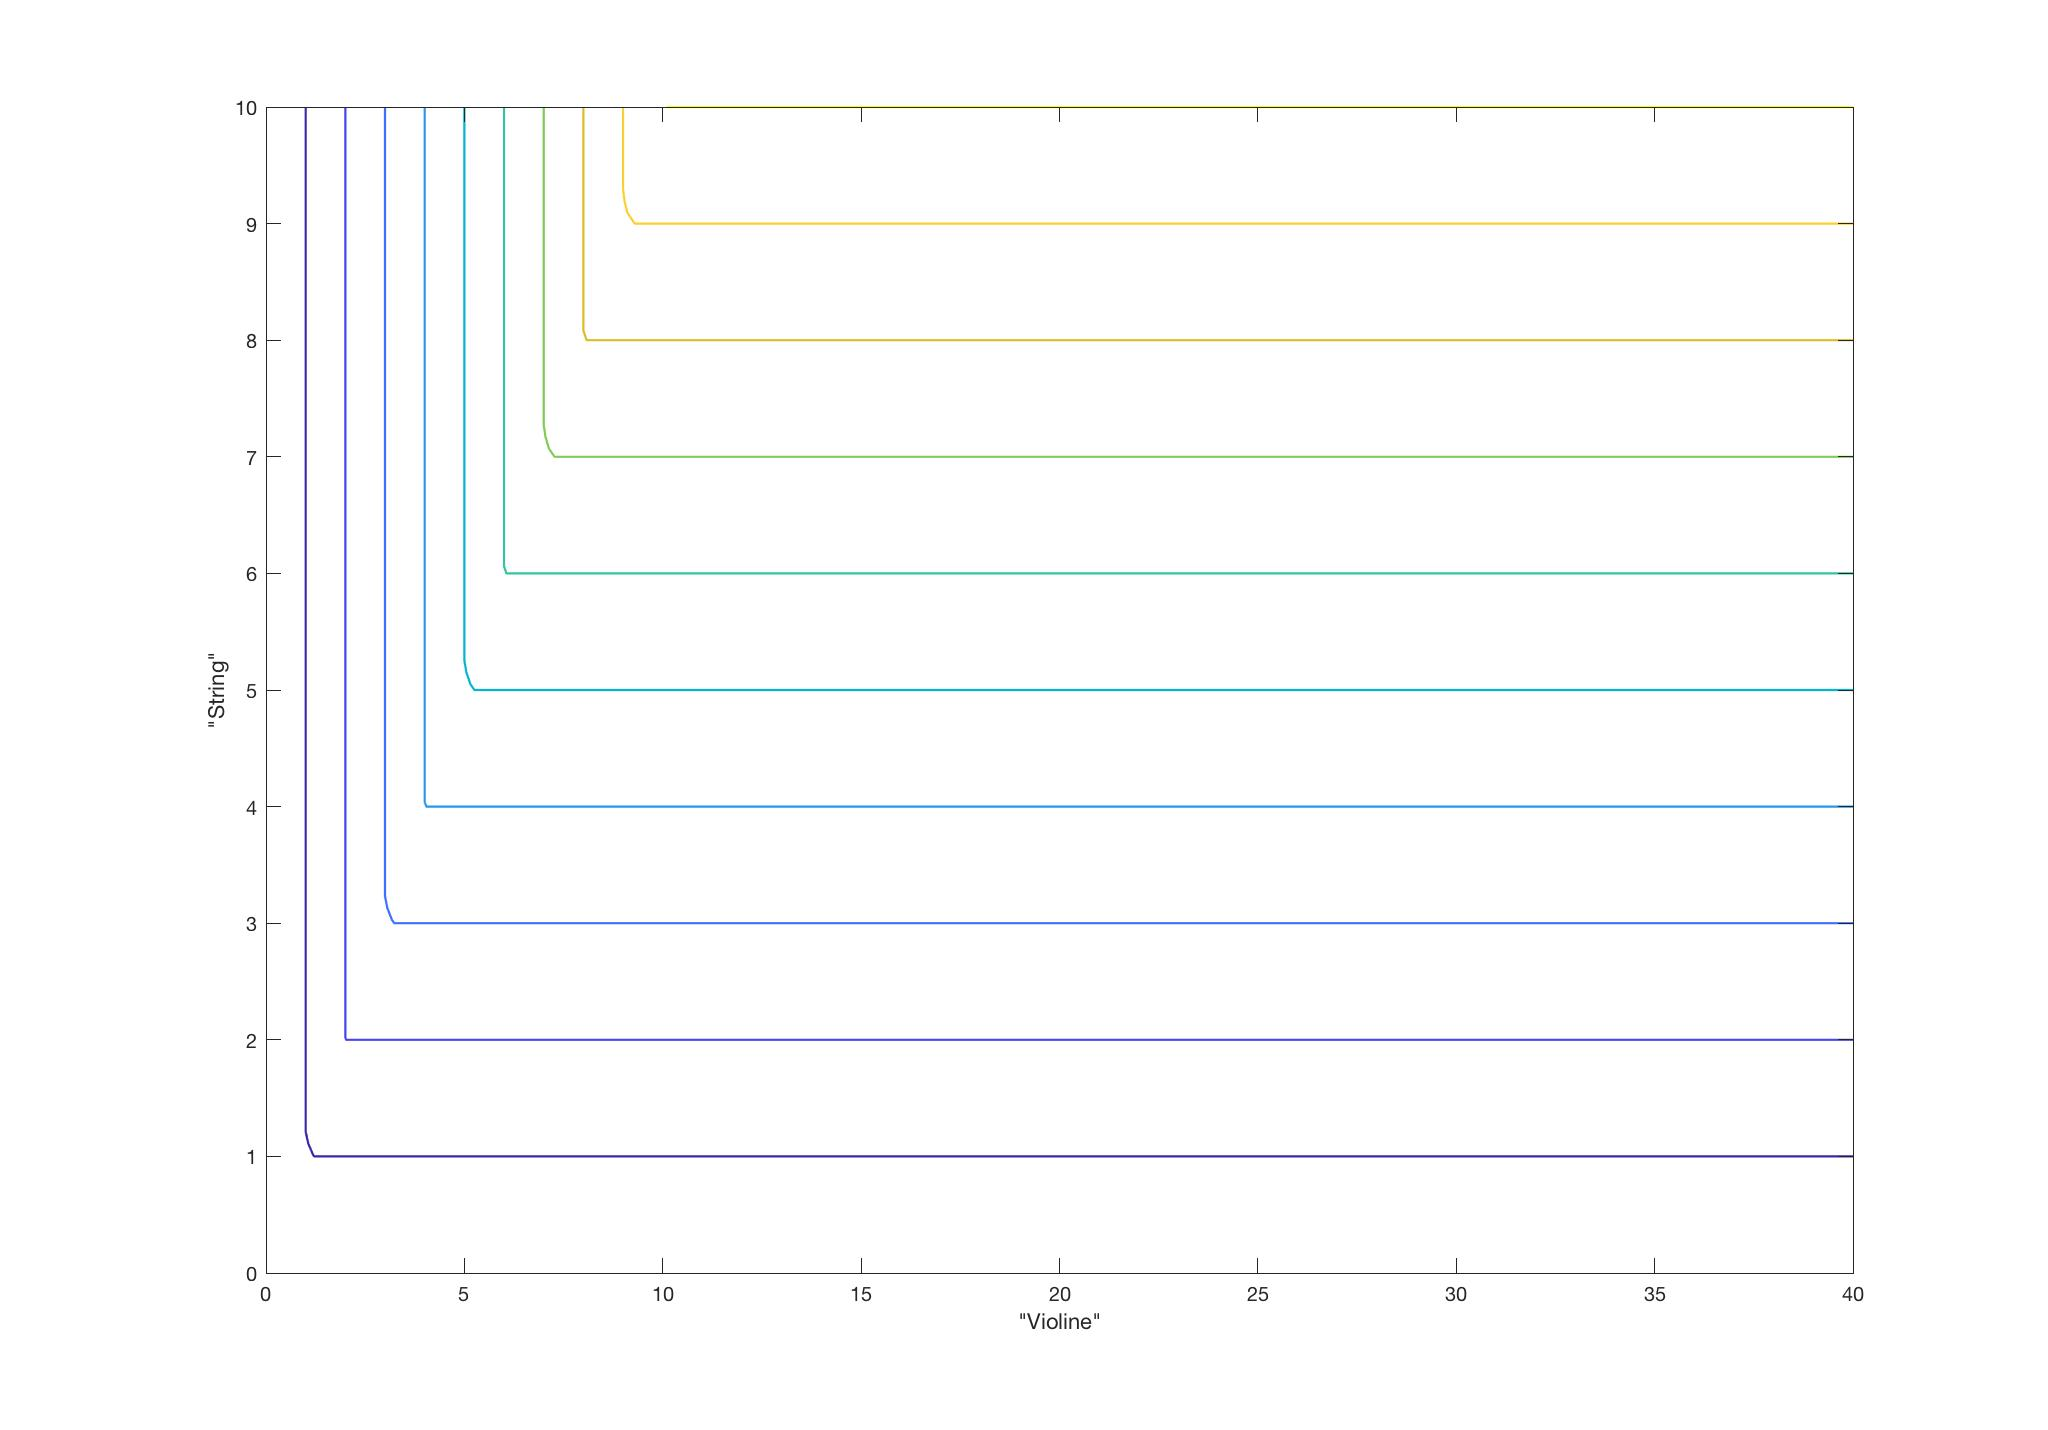
\includegraphics[width=0.8\linewidth]{eco206pic/perf_comp.jpg}
\end{figure*}
\newline
(c) What's the MRS
\begin{enumerate}
	\item 0 if $4v>s$ (flat part)
	\item $\infty$ if $4v < s$ (vertical part)
	\item \emph{undefined} on kink point
\end{enumerate}

\paragraph{Exercise2 (homothetic)} Calculate MRS when $u(x_1, x_2) = x_1 ^ \alpha x_2 ^ \beta$
\begin{multline*}
	\emph{Solution.} \\
	\pd{u}{x_1} = \alpha x_1 ^ {\alpha - 1} x_2 ^ \beta \\
	\pd{u}{x_2} = \beta x_1 ^ \alpha x_2 ^ {\beta - 1} \\
	MRS = -\frac{\pd{u}{x_1}}{\pd{u}{x_2}} = - \frac{\alpha x_2}{\beta x_1} \\
	\tx{Check convexity holds:} \\
	\tx{Method 1: Check convexity.} \\
	\tx{Method 2: Quasi-concave utility function.} \\
	\blacksquare
\end{multline*}

\paragraph{Exercise 3 (quasi-linear)} Calculate MRS if $u(x_1, x_2) = \sqrt{x_1} + x_2$
\begin{multline*}
	\emph{Solution.} \\
	MRS = - \frac{\pd{u}{x}}{\pd{u}{y}} = -\frac{0.5}{\sqrt{x_1}} \\
	\tx{Check convexity: check if absolute value of MRS diminish} \\
	\vert MRS \vert = \frac{0.5}{\sqrt{x_1}} \\
	\frac{d \vert MRS \vert}{d x_1} < 0 \tx{ for } x_1 > 0 \\
	\blacksquare
\end{multline*}

\paragraph{Exercise 4 (perfect substitute)} A consumer considers pepsi(p) and cocacola(c) as perfect substitute and is willing to exchange 0.5 can of p for 1 can of c. What is a utility function for her preference?

\begin{multline*}
	\emph{Solution.} \\
	MRS = -0.5 = - \frac{dp}{dc} = - \frac{\pd{u}{c}}{\pd{u}{p}}\\
	\implies 0.5 \pd{u}{p} = \pd{u}{c} \\
	\implies \pd{u}{p} = 2 \pd{u}{c} \\
	u(c, p) = 2 p + c \tx{ (not unique)}\\
	\blacksquare
\end{multline*}

\paragraph{Exercise (linear, corner solution)} Consider optimization problem 
\begin{multline*}
	\\
	\max_{x,y} u(x,y) = 3x+2y \\
	s.t.\ 2x + 5y = 100 \\
\end{multline*}
Solution $(x^*, y^*) = (50, 0)$

\paragraph{Exercise (Concave, corner solution)}
\begin{multline*}
	\\
	\max_{x, y} u(x,y) = x^2 + y^2 \\
	s.t.\ x + y = 100 \\
\end{multline*}
\begin{multline*}
	\emph{Solution.} \\
	\tx{Check MRS} \vert MRS \vert = \frac{dy}{dx} = \frac{x}{y} \\
	\tx{Thus increasing MRS.} \\
	\tx{Lagrange provides a minimum.} \\
	\tx{Corner solutions.} (x^*, y^*) = (0, 1000), (x^*, y^*) = (1000, 0)\\
	\blacksquare
\end{multline*}

\paragraph{Exercise (kinked budget constraint)} Suppose $u(x_1, x_2) = x_1^2 x_2^2$ and the budget constraint is defined as 
\[
	\begin{cases}
		2x_1 + x_2 = 80 \tx{ if } x_1 \leq 20 \\
		x_1 + x_2 = 60 \tx{ if } x_1 \geq 20 \\
	\end{cases}
\]
How does the optimal $x_1$ compare to 20?
\begin{multline*}
	\emph{Soluti on.} \\
	\textbf{Method 1} \\
\end{multline*}


\end{document}

































